
\section{Discussion}
\label{sec:discussion}

This section contains discussion of all the parts of this chapter, particularly the nature of the techniques employed, the nature of the mechanisms discovered and the experimental effectiveness in the context of synthetic data.
\begin{itemize}
\item	in subsection \ref{subsection:discussion_EBB} we discuss the nature and effectiveness of our derived EBB from section \ref{section:new_EBB}.
\item	in subsection \ref{subsection:main_discussion} we discuss the performance of our new SEBM method, in the context of synthetic data
\item	in subsection \ref{subsection:discussion_shapley} we discuss the performance of our SEBM method in the context of sampling the Shapley Value.
\item	in subsection \ref{sec:multi} we give indication of future work regarding the extension of SEBB to multidimensional data.
\end{itemize}



\subsection{The effectiveness of our new EBB}\label{subsection:discussion_EBB}

In section \ref{section:new_EBB} we went through the process of deriving an EBB using complex components thus yielding a requirement for numerical determination.
The resulting numerical EBB was then fitted with a symbolic envelope for ease of use - per equation \ref{eq:prob_bound}.

It is perhaps interesting to compare the strength of the new EBB against other EBBs, particularly we considered that most of the elements in our new EBB were improvements apon the process used in the derivation of Maurer and Pontil's EBB.

And so we compared our EBB directly with \cite{Maurer50empiricalbernstein}'s EBB given by theorem \ref{MandPsEBB} as:
$$\p\left(\mu-\hat{\mu}\ge\sqrt{\frac{2\hat{\sigma}^2\log(2/t)}{n}}+\frac{7D\log(2/t)}{3(n-1)}\right)\le t$$
We felt that it would only be fair to compare our EBB to Maurer and Pontil's EBB if they had applied Popoviciu's inequality as an appropriate domain restriction and carried it through their derivation, as we did to our own EBB. 
Specifically, this is the domain where:
\[ \frac{1}{2}>\frac{\sqrt{\hat{\sigma}^2}}{D}+\sqrt{\frac{2\log(2/t)}{n-1}} \]
We plotted the improvement our EBB offers in this domain, as shown in Figure \ref{biggraph3}. 

In this plot, a probability 0.5 bound is shown to shrink by approximately one third.
And we observed that our refinement of Maurer and Pontil's EBB was uniformly tighter across a large range of values.


\begin{figure}[]{}
    \centering
	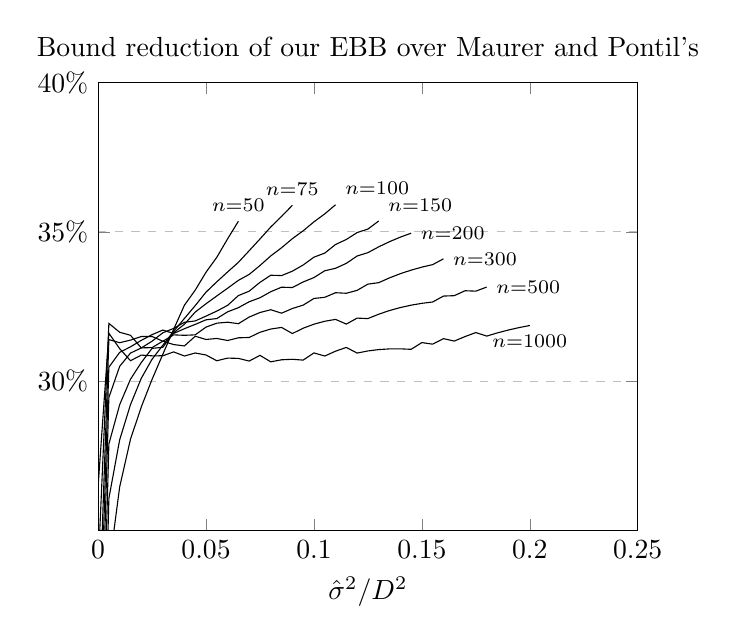
\begin{tikzpicture}
	\begin{axis}[
		title={Bound reduction of our EBB over  Maurer and Pontil's},
		xlabel={$\hat{\sigma}^2/D^2$},
		xmin=0, xmax=0.25,
		ymin=25, ymax=40,
		xtick={0,0.05,0.1,0.15,0.2,0.25},
		ytick={30,35,40},
		yticklabel=$\pgfmathprintnumber{\tick}\%$,
		ymajorgrids=true,
		grid style=dashed,
		xticklabel style={/pgf/number format/fixed},
	]
	\addplot[] coordinates {
(0.0, 10.038489469957923)(0.005, 23.729228874038338)(0.01, 26.46795119155083)(0.015, 28.061119743643296)(0.02, 29.141938583623652)(0.025, 30.066155991693723)(0.03, 30.907282335052788)(0.035, 31.738722848538305)(0.04, 32.54914392836502)(0.045, 33.05291848928947)(0.05, 33.651509619741496)(0.055, 34.151805087746446)(0.06, 34.768247610158575)(0.065, 35.35764746719292)
		}node[pos=1.0](endofplotsquare){} ;
	\node [above] at (endofplotsquare) {$\scriptstyle n=50$};
	\addplot[] coordinates {
(0.0, 12.591458904845746)(0.005, 26.08582516018055)(0.01, 28.044488963240152)(0.015, 29.219014176778845)(0.02, 30.101019545112305)(0.025, 30.739739304373572)(0.03, 31.209391146592484)(0.035, 31.67459564986504)(0.04, 32.10560417423678)(0.045, 32.53522214247566)(0.05, 32.98480753922602)(0.055, 33.33123349968554)(0.06, 33.66064263107598)(0.065, 33.983296057116895)(0.07, 34.371432119724126)(0.075, 34.76400092304011)(0.08, 35.165771922230526)(0.085, 35.51929445366766)(0.09, 35.890640326573575)
		}node[pos=1.0](endofplotsquare){} ;
	\node [above] at (endofplotsquare) {$\scriptstyle n=75$};
	\addplot[] coordinates {
(0.0, 14.817995440815901)(0.005, 27.90751007185735)(0.01, 29.219819451516923)(0.015, 30.070639062533996)(0.02, 30.629290720122317)(0.025, 31.104197838170627)(0.03, 31.14038996461402)(0.035, 31.62526607199946)(0.04, 31.911575841232846)(0.045, 32.3187069670152)(0.05, 32.59698646227685)(0.055, 32.85814963311234)(0.06, 33.115830685662)(0.065, 33.379908028841236)(0.07, 33.578110917203176)(0.075, 33.87653264786374)(0.08, 34.19803078792182)(0.085, 34.470564003329045)(0.09, 34.774201537103245)(0.095, 35.03784322660741)(0.1, 35.337583634279)(0.105, 35.60362789769355)(0.11, 35.90890662248758)
		}node[pos=1.0](endofplotsquare){} ;
	\node [above right] at (endofplotsquare) {$\scriptstyle n=100$};
	\addplot[] coordinates {
(0.0, 17.342661445161745)(0.005, 29.461247776997926)(0.01, 30.502124709956824)(0.015, 30.94634600450878)(0.02, 31.116833768989828)(0.025, 31.344627574353588)(0.03, 31.62499327739429)(0.035, 31.772139980592)(0.04, 31.975727165299386)(0.045, 32.02196228998142)(0.05, 32.183034431467235)(0.055, 32.352369659168474)(0.06, 32.54250416890406)(0.065, 32.87047963677422)(0.07, 33.017679271803296)(0.075, 33.31333732160584)(0.08, 33.55087101615144)(0.085, 33.53938459819124)(0.09, 33.68714872653657)(0.095, 33.89275583281304)(0.1, 34.15600891069251)(0.105, 34.290920495879966)(0.11, 34.57974857223946)(0.115, 34.747357884723435)(0.12, 34.97811379083637)(0.125, 35.09584827017029)(0.13, 35.36531839253051)
		}node[pos=1.0](endofplotsquare){} ;
	\node [above right] at (endofplotsquare) {$\scriptstyle n=150$};
	\addplot[] coordinates {
(0.0, 19.269181617386778)(0.005, 30.47328215171227)(0.01, 30.970505248952783)(0.015, 31.155076903228505)(0.02, 31.370737591330126)(0.025, 31.563153411429678)(0.03, 31.716924278688328)(0.035, 31.602163041853583)(0.04, 31.762160711176872)(0.045, 31.905759719654245)(0.05, 32.05956774531062)(0.055, 32.101874254626836)(0.06, 32.32639539364612)(0.065, 32.465858041087344)(0.07, 32.663895247621326)(0.075, 32.797586647322234)(0.08, 32.99998541625402)(0.085, 33.15092115439265)(0.09, 33.13907818080335)(0.095, 33.32527974281349)(0.1, 33.47347491095124)(0.105, 33.70030345616673)(0.11, 33.78337094262078)(0.115, 33.94866206353597)(0.12, 34.19406008169977)(0.125, 34.30666804274627)(0.13, 34.5014054670121)(0.135, 34.67351335871075)(0.14, 34.82497129829329)(0.145, 34.95753413863828)
		}node[pos=1.0](endofplotsquare){} ;
	\node [right] at (endofplotsquare) {$\scriptstyle n=200$};
	\addplot[] coordinates {
(0.0, 21.01455983414305)(0.005, 31.398323351742654)(0.01, 31.29316800287044)(0.015, 31.380044700971307)(0.02, 31.499573558604126)(0.025, 31.501955199548522)(0.03, 31.342388805161228)(0.035, 31.555898653589576)(0.04, 31.540720961712708)(0.045, 31.556719994430246)(0.05, 31.815518124296712)(0.055, 31.947447662218103)(0.06, 31.979020008525413)(0.065, 31.929950573976118)(0.07, 32.151946530365926)(0.075, 32.30372613153442)(0.08, 32.39631985663968)(0.085, 32.28147349936643)(0.09, 32.43775937546441)(0.095, 32.55064623256504)(0.1, 32.77372870056995)(0.105, 32.81284419609248)(0.11, 32.96572615770543)(0.115, 32.94748952790814)(0.12, 33.04474761150041)(0.125, 33.25359991684834)(0.13, 33.30204392434083)(0.135, 33.462830030160355)(0.14, 33.601886363972085)(0.145, 33.7211101175424)(0.15, 33.822185822075845)(0.155, 33.90661477833436)(0.16, 34.09961256888578)
		}node[pos=1.0](endofplotsquare){} ;
	\node [right] at (endofplotsquare) {$\scriptstyle n=300$};
	\addplot[] coordinates {
(0.0, 23.733576061543907)(0.005, 31.93999128292596)(0.01, 31.642400396531094)(0.015, 31.54212092349261)(0.02, 31.12052542652318)(0.025, 31.129819611252405)(0.03, 31.344098301521242)(0.035, 31.231838999520004)(0.04, 31.185453514912005)(0.045, 31.51029078782499)(0.05, 31.401697787018254)(0.055, 31.43592520457107)(0.06, 31.367624957687056)(0.065, 31.45753767654653)(0.07, 31.468778394474676)(0.075, 31.6423499409508)(0.08, 31.751037287923307)(0.085, 31.804794091938522)(0.09, 31.59991862434968)(0.095, 31.778311022724473)(0.1, 31.913384999263183)(0.105, 32.010501900631745)(0.11, 32.074189915872516)(0.115, 31.915973789453584)(0.12, 32.11613625130849)(0.125, 32.10053700848796)(0.13, 32.24708311545571)(0.135, 32.3692691037866)(0.14, 32.46936498795406)(0.145, 32.54937215145163)(0.15, 32.61106237732128)(0.155, 32.65601018366708)(0.16, 32.85390573088976)(0.165, 32.867317678660584)(0.17, 33.03199624865481)(0.175, 33.01872182909822)(0.18, 33.15487119563348)
		}node[pos=1.0](endofplotsquare){} ;
	\node [right] at (endofplotsquare) {$\scriptstyle n=500$};
	\addplot[] coordinates {
(0.0, 26.48466951022569)(0.005, 31.610541001763814)(0.01, 31.094245131329373)(0.015, 30.691021818068354)(0.02, 30.878933354114203)(0.025, 30.854623560301786)(0.03, 30.855718952687877)(0.035, 30.985476785778605)(0.04, 30.84839664811395)(0.045, 30.94907807084863)(0.05, 30.882232292715344)(0.055, 30.68950445827823)(0.06, 30.77857995587979)(0.065, 30.768677505684852)(0.07, 30.679146150855704)(0.075, 30.870441770906094)(0.08, 30.653781659199446)(0.085, 30.72198559607093)(0.09, 30.738566645167236)(0.095, 30.710992728150178)(0.1, 30.95229310334558)(0.105, 30.847606478652455)(0.11, 31.009527688997892)(0.115, 31.135832380489546)(0.12, 30.946326663430018)(0.125, 31.017664917855072)(0.13, 31.06348584444511)(0.135, 31.08638415275851)(0.14, 31.0886271157673)(0.145, 31.072204850949028)(0.15, 31.29715291414822)(0.155, 31.244828197450204)(0.16, 31.429852460842593)(0.165, 31.347766957340134)(0.17, 31.49894525891586)(0.175, 31.63356906325342)(0.18, 31.514234978296805)(0.185, 31.62214364046394)(0.19, 31.716729481001114)(0.195, 31.79891328121711)(0.2, 31.869534804168858)
		}node[pos=1.0](endofplotsquare){} ;
	\node [below] at (endofplotsquare) {$\scriptstyle n=1000$};
	\end{axis}
	\end{tikzpicture}
	\vspace{-10pt}
	\caption[The percent reduction our EBB would achieve]{The percent reduction of the 0.5 probability bound, that going from Maurer and Pontil's EBB to our EBB would achieve, for various $n$, in the domain valid for their EBB.}
	\label{biggraph3}
	
	
	\vspace{15pt}
	
	
	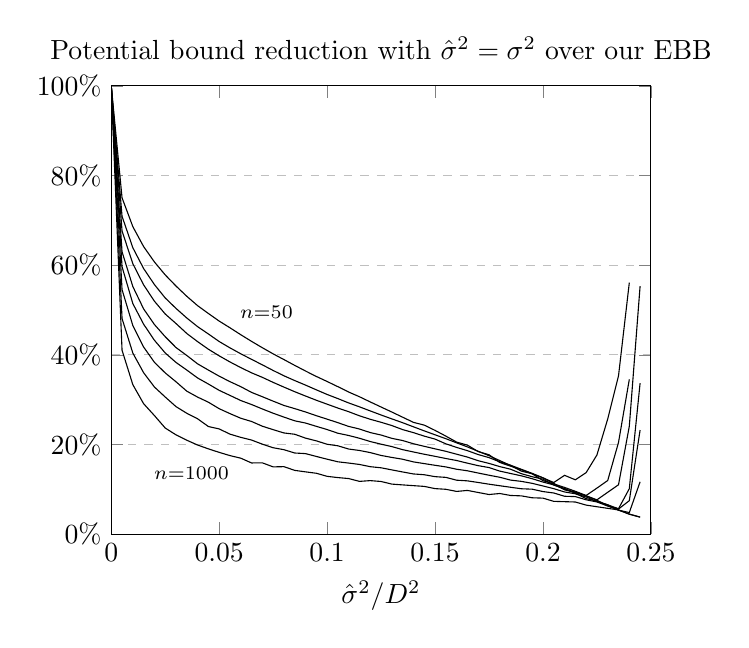
\begin{tikzpicture}
	\begin{axis}[
		title={Potential bound reduction with $\hat{\sigma}^2 = \sigma^2$ over our EBB},
		xlabel={$\hat{\sigma}^2/D^2$},
		xmin=0, xmax=0.25,
		ymin=0, ymax=100,
		xtick={0,0.05,0.1,0.15,0.2,0.25},
		ytick={0,20,40,60,80,100},
		yticklabel=$\pgfmathprintnumber{\tick}\%$,
		legend pos=south west,
		ymajorgrids=true,
		grid style=dashed,
		xticklabel style={/pgf/number format/fixed},
	]
	\addplot[] coordinates {
(0.0, 100.0)(0.005, 75.02420135527589)(0.01, 68.58202038924931)(0.015, 64.13237924865832)(0.02, 60.71118820468343)(0.025, 57.819103972950124)(0.03, 55.33498759305211)(0.035, 53.04630381803412)(0.04, 50.96)(0.045, 49.21383647798742)(0.05, 47.51937984496124)(0.055, 46.02446483180428)(0.06, 44.47806354009077)(0.065, 42.99625468164794)(0.07, 41.57386785449146)(0.075, 40.20618556701031)(0.08, 38.93352812271731)(0.085, 37.63596809282088)(0.09, 36.38328530259366)(0.095, 35.17191977077364)(0.1, 34.04558404558404)(0.105, 32.88447909284196)(0.11, 31.68666196189132)(0.115, 30.639494026704146)(0.12, 29.481792717086833)(0.125, 28.35195530726257)(0.13, 27.228412256267408)(0.135, 26.0778859527121)(0.14, 24.930555555555557)(0.145, 24.31129476584022)(0.15, 23.140495867768596)(0.155, 21.862068965517242)(0.16, 20.525224602626125)(0.165, 19.8489010989011)(0.17, 18.413793103448278)(0.175, 17.707618393960193)(0.18, 15.975103734439834)(0.185, 15.161957270847692)(0.19, 14.36426116838488)(0.195, 13.452299245024022)(0.2, 12.542837559972584)(0.205, 11.51473612063057)(0.21, 13.115845539280958)(0.215, 12.117177097203728)(0.22, 13.71280724450194)(0.225, 17.65424557116677)(0.23, 25.69558101472995)(0.235, 35.30794546309356)(0.24, 56.085994309200125)
		}node[pos=0.4](endofplotsquare){} ;
	\node [above right] at (endofplotsquare) {$\scriptstyle n=50$};
	\addplot[] coordinates {
(0.0, 100.0)(0.005, 70.89337175792507)(0.01, 63.881401617250674)(0.015, 59.23076923076923)(0.02, 55.66502463054187)(0.025, 52.67538644470868)(0.03, 50.345622119815665)(0.035, 48.20627802690583)(0.04, 46.2800875273523)(0.045, 44.646680942184155)(0.05, 42.96218487394958)(0.055, 41.54639175257732)(0.06, 40.22289766970618)(0.065, 38.983050847457626)(0.07, 37.75811209439528)(0.075, 36.50485436893204)(0.08, 35.31669865642994)(0.085, 34.25047438330171)(0.09, 33.23943661971831)(0.095, 32.18604651162791)(0.1, 31.152073732718893)(0.105, 30.228310502283104)(0.11, 29.257246376811594)(0.115, 28.39173405211141)(0.12, 27.475468331846567)(0.125, 26.572187776793623)(0.13, 25.704225352112676)(0.135, 24.84689413823272)(0.14, 23.93385552654482)(0.145, 23.03030303030303)(0.15, 22.155172413793103)(0.155, 21.28755364806867)(0.16, 20.35928143712575)(0.165, 19.453924914675767)(0.17, 18.46808510638298)(0.175, 17.502124044180118)(0.18, 16.397621070518266)(0.185, 15.306122448979592)(0.19, 14.054514480408859)(0.195, 13.463166807790008)(0.2, 11.925042589437819)(0.205, 11.205432937181664)(0.21, 10.414902624894157)(0.215, 9.551986475063398)(0.22, 8.622147083685546)(0.225, 10.262725779967159)(0.23, 11.961722488038278)(0.235, 20.45616535994298)(0.24, 34.51481696687972)
		}node[pos=0.693](endofplotsquare){} ;
	%\node [above] at (endofplotsquare) {$\scriptstyle n=75$};
	\addplot[] coordinates {
(0.0, 100.0)(0.005, 67.61904761904762)(0.01, 60.31468531468531)(0.015, 55.5921052631579)(0.02, 51.95618153364632)(0.025, 49.0990990990991)(0.03, 46.97406340057637)(0.035, 44.75524475524475)(0.04, 42.93478260869565)(0.045, 41.246684350132625)(0.05, 39.766839378238345)(0.055, 38.40304182509506)(0.06, 37.142857142857146)(0.065, 35.97560975609756)(0.07, 34.97005988023952)(0.075, 33.844339622641506)(0.08, 32.7906976744186)(0.085, 31.76605504587156)(0.09, 30.804077010192525)(0.095, 29.86577181208054)(0.1, 28.98230088495575)(0.105, 28.11816192560175)(0.11, 27.302275189599133)(0.115, 26.394849785407725)(0.12, 25.61105207226355)(0.125, 24.94736842105263)(0.13, 24.217118997912316)(0.135, 23.316062176165804)(0.14, 22.633744855967077)(0.145, 21.859039836567927)(0.15, 21.196754563894523)(0.155, 20.141700404858298)(0.16, 19.335347432024168)(0.165, 18.61861861861862)(0.17, 17.74675972083749)(0.175, 17.063492063492063)(0.18, 16.12265084075173)(0.185, 15.369458128078819)(0.19, 14.454277286135694)(0.195, 13.555992141453832)(0.2, 12.561334641805692)(0.205, 11.307767944936087)(0.21, 9.881422924901186)(0.215, 9.251968503937007)(0.22, 8.537782139352306)(0.225, 7.647058823529412)(0.23, 9.333333333333334)(0.235, 11.00832562442183)(0.24, 24.0625)(0.245, 55.32786885245902)
		}node[pos=1.0](endofplotsquare){} ;
	%\node [above] at (endofplotsquare) {$n=100$};
	\addplot[] coordinates {
(0.0, 100.0)(0.005, 62.98342541436464)(0.01, 55.223880597014926)(0.015, 50.23041474654378)(0.02, 46.753246753246756)(0.025, 44.03292181069959)(0.03, 41.61735700197239)(0.035, 39.84819734345351)(0.04, 37.981651376146786)(0.045, 36.58969804618117)(0.05, 35.233160621761655)(0.055, 34.00673400673401)(0.06, 32.89473684210526)(0.065, 31.612903225806452)(0.07, 30.647709320695103)(0.075, 29.658385093167702)(0.08, 28.702290076335878)(0.085, 27.994011976047904)(0.09, 27.245949926362297)(0.095, 26.41509433962264)(0.1, 25.644699140401148)(0.105, 24.858757062146893)(0.11, 24.022346368715084)(0.115, 23.448275862068964)(0.12, 22.646657571623464)(0.125, 22.10242587601078)(0.13, 21.36181575433912)(0.135, 20.871862615587848)(0.14, 20.157068062827225)(0.145, 19.58495460440986)(0.15, 19.02313624678663)(0.155, 18.471337579617835)(0.16, 17.825537294563844)(0.165, 17.189460476787954)(0.17, 16.375)(0.175, 15.77639751552795)(0.18, 15.061728395061728)(0.185, 14.478527607361963)(0.19, 13.480392156862745)(0.195, 12.804878048780488)(0.2, 12.257281553398059)(0.205, 10.94890510948905)(0.21, 10.194174757281553)(0.215, 9.101941747572816)(0.22, 7.907542579075426)(0.225, 7.38498789346247)(0.23, 6.521739130434782)(0.235, 5.669481302774427)(0.24, 10.136674259681094)(0.245, 33.693843594009984)
		}node[pos=1.0](endofplotsquare){} ;
	%\node [above] at (endofplotsquare) {$n=150$};
	\addplot[] coordinates {
(0.0, 100.0)(0.005, 59.642857142857146)(0.01, 51.41955835962145)(0.015, 46.820809248554916)(0.02, 43.24324324324324)(0.025, 40.40920716112532)(0.03, 38.292682926829265)(0.035, 36.5967365967366)(0.04, 34.831460674157306)(0.045, 33.47826086956522)(0.05, 32.06751054852321)(0.055, 30.942622950819672)(0.06, 29.8)(0.065, 28.90625)(0.07, 27.915869980879542)(0.075, 26.96629213483146)(0.08, 26.102941176470587)(0.085, 25.270758122743683)(0.09, 24.778761061946902)(0.095, 24.041811846689896)(0.1, 23.32761578044597)(0.105, 22.504230118443317)(0.11, 22.0)(0.115, 21.38157894736842)(0.12, 20.650406504065042)(0.125, 20.064205457463885)(0.13, 19.523809523809526)(0.135, 18.838304552590266)(0.14, 18.322981366459626)(0.145, 17.81874039938556)(0.15, 17.35159817351598)(0.155, 16.867469879518072)(0.16, 16.417910447761194)(0.165, 15.828402366863905)(0.17, 15.27165932452276)(0.175, 14.847161572052402)(0.18, 14.057971014492754)(0.185, 13.525179856115107)(0.19, 13.0)(0.195, 12.357954545454545)(0.2, 11.614730878186968)(0.205, 10.985915492957746)(0.21, 10.0)(0.215, 9.396914446002805)(0.22, 8.531468531468532)(0.225, 7.5524475524475525)(0.23, 6.3113604488078545)(0.235, 5.594405594405594)(0.24, 7.462686567164179)(0.245, 23.214285714285715)
		}node[pos=1.0](endofplotsquare){} ;
	%\node [above] at (endofplotsquare) {$n=200$};
	\addplot[] coordinates {
(0.0, 100.0)(0.005, 54.54545454545455)(0.01, 46.52173913043478)(0.015, 41.732283464566926)(0.02, 38.32116788321168)(0.025, 35.95890410958904)(0.03, 33.980582524271846)(0.035, 31.888544891640866)(0.04, 30.56379821958457)(0.045, 29.428571428571427)(0.05, 27.977839335180054)(0.055, 26.881720430107528)(0.06, 25.848563968668408)(0.065, 25.126903553299492)(0.07, 24.069478908188586)(0.075, 23.300970873786408)(0.08, 22.565320665083135)(0.085, 22.273781902552205)(0.09, 21.4123006833713)(0.095, 20.80536912751678)(0.1, 20.044052863436125)(0.105, 19.696969696969695)(0.11, 18.976545842217483)(0.115, 18.658280922431867)(0.12, 18.181818181818183)(0.125, 17.551020408163264)(0.13, 17.10261569416499)(0.135, 16.69980119284294)(0.14, 16.110019646365423)(0.145, 15.728155339805825)(0.15, 15.355086372360844)(0.155, 14.990512333965844)(0.16, 14.473684210526315)(0.165, 14.12639405204461)(0.17, 13.627992633517495)(0.175, 13.138686131386862)(0.18, 12.681159420289855)(0.185, 12.050359712230216)(0.19, 11.764705882352942)(0.195, 11.327433628318584)(0.2, 10.73943661971831)(0.205, 10.13986013986014)(0.21, 9.40766550522648)(0.215, 8.996539792387543)(0.22, 8.290155440414507)(0.225, 7.253886010362694)(0.23, 6.540447504302926)(0.235, 5.344827586206897)(0.24, 4.810996563573883)(0.245, 11.67192429022082)
		}node[pos=1.0](endofplotsquare){} ;
	%\node [above] at (endofplotsquare) {$n=300$};
	\addplot[] coordinates {
(0.0, 100.0)(0.005, 48.091603053435115)(0.01, 40.38461538461539)(0.015, 36.0)(0.02, 32.8125)(0.025, 30.58252427184466)(0.03, 28.440366972477065)(0.035, 26.956521739130434)(0.04, 25.726141078838175)(0.045, 24.0)(0.05, 23.46153846153846)(0.055, 22.304832713754646)(0.06, 21.58273381294964)(0.065, 20.97902097902098)(0.07, 20.068027210884352)(0.075, 19.269102990033222)(0.08, 18.83116883116883)(0.085, 18.095238095238095)(0.09, 17.956656346749227)(0.095, 17.325227963525837)(0.1, 16.71641791044776)(0.105, 16.129032258064516)(0.11, 15.85014409221902)(0.115, 15.536723163841808)(0.12, 15.041782729805014)(0.125, 14.794520547945206)(0.13, 14.324324324324325)(0.135, 13.866666666666667)(0.14, 13.421052631578947)(0.145, 13.246753246753247)(0.15, 12.820512820512821)(0.155, 12.658227848101266)(0.16, 12.030075187969924)(0.165, 11.881188118811881)(0.17, 11.519607843137255)(0.175, 11.138014527845037)(0.18, 10.79136690647482)(0.185, 10.451306413301662)(0.19, 10.117647058823529)(0.195, 10.023310023310023)(0.2, 9.49074074074074)(0.205, 9.174311926605505)(0.21, 8.447488584474886)(0.215, 8.371040723981901)(0.22, 7.657657657657658)(0.225, 7.174887892376682)(0.23, 6.263982102908278)(0.235, 5.369127516778524)(0.24, 4.464285714285714)(0.245, 3.7861915367483294)
		}node[pos=1.0](endofplotsquare){} ;
	%\node [above] at (endofplotsquare) {$n=500$};
	\addplot[] coordinates {
(0.0, 100.0)(0.005, 41.02564102564103)(0.01, 33.333333333333336)(0.015, 29.09090909090909)(0.02, 26.446280991735538)(0.025, 23.66412213740458)(0.03, 22.142857142857142)(0.035, 20.945945945945947)(0.04, 19.871794871794872)(0.045, 19.01840490797546)(0.05, 18.235294117647058)(0.055, 17.51412429378531)(0.06, 16.939890710382514)(0.065, 15.873015873015873)(0.07, 15.897435897435898)(0.075, 15.0)(0.08, 15.048543689320388)(0.085, 14.218009478672986)(0.09, 13.88888888888889)(0.095, 13.574660633484163)(0.1, 12.88888888888889)(0.105, 12.608695652173912)(0.11, 12.393162393162394)(0.115, 11.764705882352942)(0.12, 11.934156378600823)(0.125, 11.740890688259109)(0.13, 11.155378486055778)(0.135, 10.980392156862745)(0.14, 10.81081081081081)(0.145, 10.64638783269962)(0.15, 10.150375939849624)(0.155, 10.0)(0.16, 9.523809523809524)(0.165, 9.747292418772563)(0.17, 9.285714285714286)(0.175, 8.8339222614841)(0.18, 9.059233449477352)(0.185, 8.620689655172415)(0.19, 8.532423208191126)(0.195, 8.108108108108109)(0.2, 8.02675585284281)(0.205, 7.308970099667774)(0.21, 7.2368421052631575)(0.215, 7.166123778501628)(0.22, 6.472491909385114)(0.225, 6.109324758842444)(0.23, 5.7507987220447285)(0.235, 5.396825396825397)(0.24, 4.444444444444445)(0.245, 3.7974683544303796)
		}node[pos=0.85](endofplotsquare){} ;
	\node [below left] at (endofplotsquare) {$\scriptstyle n=1000$};
	\end{axis}
	\end{tikzpicture}
	\vspace{-10pt}
	\caption[The percent reduction our EBB could yet achieve]{The percent reduction in the 0.5 probability bound that going from our EBB to using Bennett's inequality (perfect variance information, $\hat{\sigma}^2 = \sigma^2$) achieves, for $n=50,75,100,150,200,300,500,1000$.}
	\label{biggraph4}
\end{figure}


While this may be an interesting result, we also sought to put this in perspective with what could ideally be achieved
And so we conducted a comparison about the further improvement over our EBB that might be achieved with perfect information about the variance; specifically that, Bennett's inequality is used assuming $\hat{\sigma}^2=\sigma^2$.
The improvement that Bennett's inequality (with perfect variance information) has over our EBB is plotted in Figure \ref{biggraph4}, which shows that when the variance is small, uncertainty about the variance is the most detrimental to an EBB, such as ours.
However, it is witnessed that loosely going from our EBB to perfect variance information shrinks the bound by about another third.
In this way (although the results are loose) we can witness that our EBB provides approximately a half-way mark from existing state-of-the-art EBBs to an impossible ideal of having perfect variance information.

The purpose of developing a stronger EBB was to see if it could be used to improve the selection of samples in the context of stratified sampling (particularly of the Shapley Value) over other EBBs.
It was expected that the better and more tight the EBBs used, the more likely it would be that iteratively choosing samples to minimise such a bound would produce better sample choices and thus yield better estimate of the population mean.

And while it is evident that the EBB we produced was tighter than Maurer and Pontil's EBB, the actual resulting performance difference between (as seen between \textsc{EEBB} and \textsc{Maurer} in Table \ref{Table1}) is surprisingly marginal; so marginal infact it is comparable against the performance of using unioned Hoeffding bounds - as \textsc{Hoeffding} method.
We continue discussion of this surprising result in the context of all the other methods in section \ref{subsection:main_discussion}.



\subsection{Discussion of stratified sampling results}\label{subsection:main_discussion}


The results for our different sampling methods are shown across Figures~\ref{Table1},\ref{Table111} and \ref{biggraph3}, with the main observation that most of the techniques performed well and similar to Neyman sampling, and that our sampling technique (including SEBM (or SEBM-W) and SECM) performed competitively to Neyman sampling (\textsc{Ney} or \textsc{Ney-W}) despite not having access to knowledge of strata variances.

It is also observed that Neyman sampling was ultimately the most accurate, for reasons that were hinted in section \ref{sec:neyman_sampling}.
Particularly that if sufficient samples have been taken then the sample means of the strata will tend to approximately be Gaussian distributed by the Central Limit Theorem.
In this context the strata means have a distribution that is entirely characterised by their mean and variance, and hence so too is the population mean estimate.
Thus the variance of the sampled population mean is the only parameter determining its error, and minimising it directly translates into improved accuracy.
The fact that the variances of the strata are the only parameters determining the error in the stratified sampling process is most directly exploited by Neyman allocation but is more obscured in SEBM* allocation methodology (as it is based only on a simplification of Bennett's inequality), thus leading to slightly worse results, particularly in Figure \ref{biggraph3}.

However this mode of explanation is perhaps the underlying reason for the similarity in performance of many of the other methods as well, particularly that after sufficiently many samples have been taken the sample means of all of the strata become Gaussian distributed and the performance of the methods then depend primarily on how effectively they estimate the variances of the strata and then allocate accordingly.
Perhaps in our Beta synthetic data there was not sufficient spread of data variances for it to make significant difference how effectively this variance estimation and allocation was done.

%One of the most remarkable inferences from the data is just how very readily Central Limit Theorem dynamics emerges, from Figure \ref{fig:central_limit_theorem} we can see that the sample error of uniformly distributed data converges almost perfectly to a gaussian distribution even in just 4 samples.

Conversely the Bernoulli-uniform synthetic data was specifically designed to create a significant spread in variance between the strata.
And the results (plotted in \ref{biggraph3}) reveal the design to amplify the detriment in stratified sampling that uncertainty about the variances would yield.
In this context Neyman sampling is very efficient as it samples based on perfect variance information, and reversely our method SEBM performs worse as it extends from minimising only a simplification of Bennett's inequality under uncertainty of the variance - this is most evident in figure \ref{biggraph3}.
Because of this uncertainty about the variance, the more infrequent the Bernoulli outlier, the more likely that the methods without variance information would over-sample the Bernoulli stratum - which they did.
The relative inefficiency of the SECM method also interesting, particularly as it sought to minimise Chebyshev's inequality for the stratified sampling, and under perfect variance information would be identical to Neyman sampling.
The implication in this context is that the inefficiency of utilising these methods primarily extends from uncertainty about the variances of the strata.

From between Figures~\ref{Table1} and \ref{Table111} we observe that sampling without replacement always performs better than sampling with replacement for the same method, and this improvement is magnified as the number of samples grows large relative to the size of the population. 
At the same time, simple \textsc{Random} sampling almost always performs worst, because it fails to take advantage of any variance information, and \textsc{Simple} sampling performs even worse as it fails to take into account data stratification, these results are as expected.
Therefore from the Figures ~\ref{Table1} and \ref{Table111} we see that the primary increase in performance comes from employing stratified sampling over simple sampling, sampling without replacement over sampling with replacement, and then using some method that is more intelligent than randomly selecting samples (ie. \textsc{Random} method) and preferably using stratum variance information to get close to the ideal of Neyman sampling.

Aside from comparing the different performances of these bounds as a target for minimisation by selective sampling, it also was seen to be productive to consider them on their own - simply as bounds on the stratified mean error.
Particularly we can see a range of different strengths of the bounds in Figure \ref{fig:bounds_widths}.

In Figure \ref{fig:bounds_widths} we have plotted the bound widths of the various probability bounds of this paper in the context of the Beta-distributed data we considered in section \ref{sec:beta_distributed_data} achieved after a sample budget $n=50N$ samples allocated using \textsc{Ney-W} method.
In this graph we considered the following bounds for the error:

\begin{itemize}
\item 
\textsc{Ney-B} The bound attained using knowledge of the variances of the strata using Chebyshev's inequality (Theorem \ref{thm:chebyshevs}) in conjunction with the additivity of variance rule (Equation \ref{eq:variance_decomposition_for_strata_mean})
\item 
\textsc{SEBB*} The bound of Theorem \ref{thm:1} with variance knowledge of the variances, also using sampling without replacement sharpening (Theorem \ref{martingale0}) where optimal.
\item 
\textsc{SEBB*-W} The bound of Theorem \ref{thm:1} with variance knowledge of the variances, not using sampling without replacement sharpening (Theorem \ref{martingale0}).
\item 
\textsc{SECB} The bound of Theorem \ref{thm:SECM_bound}, which utilises Chebyshev's inequality together with our probability bound on error deviation.
\item 
\textsc{SEBB} The bound of Theorem \ref{thm:SEBM_bound}, using sampling without replacement sharpening (Theorem \ref{martingale0}) where optimal.
\item 
\textsc{SEBB-W} The bound of Theorem \ref{thm:SEBM_bound}, not sampling without replacement sharpening (Theorem \ref{martingale0}).
\item 
\textsc{Hoeffding-B} The bound attained by Hoeffding's inequality (Theorem \ref{Hoeffdings_inequality_proper}) for the strata, unioned together (via Theorem \ref{triangle_theorem2}) to create a bound on the stratified sampling error.
\item 
\textsc{Audibert-B} The bound attained by Audibert et.al's EBB inequality (Theorem \ref{AudibertsEBB}) for the strata, unioned together (via Theorem \ref{triangle_theorem2}) to create a bound on the stratified sampling error.
\item 
\textsc{Maurer-B} The bound attained by Maurer and Pontil's EBB inequality (Theorem \ref{MandPsEBB}) for the strata, unioned together (via Theorem \ref{triangle_theorem2}) to create a bound on the stratified sampling error.
\end{itemize}

Particularly we see from Figure \ref{fig:bounds_widths} that tightest bounds are given by those methods which are rooted in perfect variance information, and the widest bounds are given by those methods which utilise probability unions to bind EBBs together (via Theorem \ref{triangle_theorem2}).
What is most notable is the dissimilarity between the widths of the bounds and their effectiveness as a target for sampling minimisation; as choosing samples to minimise a probability bound is sensitive to the shape of the bound not its magnitude.
Also comparing this Figure \ref{fig:bounds_widths}, with Figures \ref{Table1},\ref{Table111} we can see that the width of the bounds are much wider than the magnitudes of the error which are actually achieved; and this is quite expected, as analytic concentration inequalities function generally as conservative confidence intervals on the error of sampling.

%
    \begin{figure}[]
        \centering
		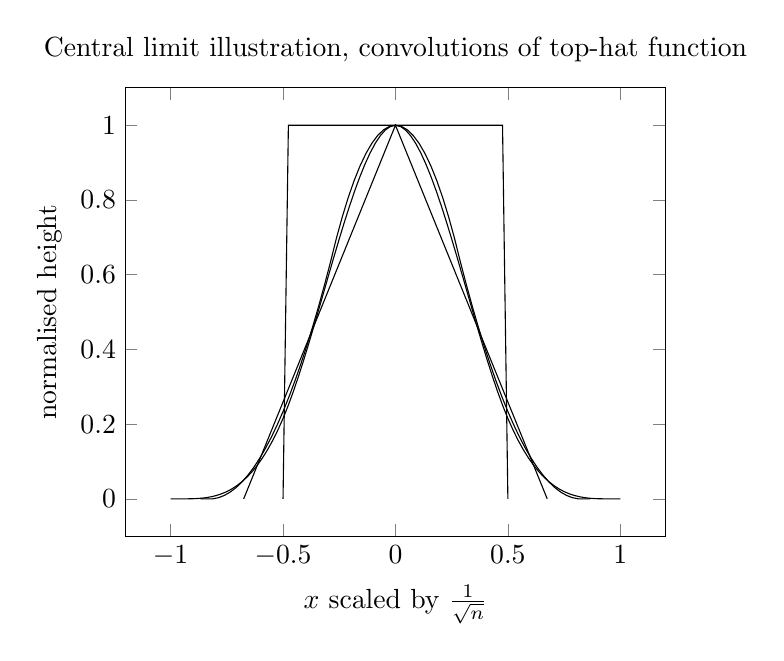
\begin{tikzpicture}
		\begin{axis}[
			title={Central limit illustration, convolutions of top-hat function},
			xlabel={$x$ scaled by $\frac{1}{\sqrt{n}}$},
			ylabel={normalised height},
		]
		\addplot[black] coordinates {
(-0.5, 0.0)(-0.47619047619047616, 1.0)(-0.4523809523809524, 1.0)(-0.4285714285714286, 1.0)(-0.40476190476190477, 1.0)(-0.38095238095238093, 1.0)(-0.35714285714285715, 1.0)(-0.33333333333333337, 1.0)(-0.30952380952380953, 1.0)(-0.2857142857142857, 1.0)(-0.2619047619047619, 1.0)(-0.23809523809523808, 1.0)(-0.2142857142857143, 1.0)(-0.19047619047619047, 1.0)(-0.16666666666666669, 1.0)(-0.14285714285714285, 1.0)(-0.11904761904761907, 1.0)(-0.09523809523809523, 1.0)(-0.07142857142857145, 1.0)(-0.047619047619047616, 1.0)(-0.023809523809523836, 1.0)(0.0, 1.0)(0.023809523809523836, 1.0)(0.04761904761904767, 1.0)(0.0714285714285714, 1.0)(0.09523809523809523, 1.0)(0.11904761904761907, 1.0)(0.1428571428571429, 1.0)(0.16666666666666663, 1.0)(0.19047619047619047, 1.0)(0.2142857142857143, 1.0)(0.23809523809523814, 1.0)(0.26190476190476186, 1.0)(0.2857142857142857, 1.0)(0.30952380952380953, 1.0)(0.33333333333333337, 1.0)(0.3571428571428571, 1.0)(0.38095238095238093, 1.0)(0.40476190476190477, 1.0)(0.4285714285714286, 1.0)(0.45238095238095233, 1.0)(0.47619047619047616, 1.0)(0.5, 0.0)
        }node[pos=0.91](endofplotsquare){} ;
		%\node [below,color={rgb:red,0;green,0;yellow,0}] at (endofplotsquare) {\footnotesize Our Bound};
		\addplot[black] coordinates {
(-0.6749655638598864, 0.0)(-0.6428243465332251, 0.047619047619047616)(-0.6106831292065639, 0.09523809523809523)(-0.5785419118799026, 0.14285714285714285)(-0.5464006945532413, 0.19047619047619047)(-0.51425947722658, 0.23809523809523808)(-0.48211825989991886, 0.2857142857142857)(-0.44997704257325755, 0.3333333333333333)(-0.41783582524659624, 0.38095238095238093)(-0.385694607919935, 0.42857142857142855)(-0.3535533905932738, 0.47619047619047616)(-0.3214121732666126, 0.5238095238095238)(-0.2892709559399513, 0.5714285714285714)(-0.25712973861329, 0.6190476190476191)(-0.2249885212866288, 0.6666666666666666)(-0.1928473039599675, 0.7142857142857143)(-0.1607060866333063, 0.7619047619047619)(-0.12856486930664499, 0.8095238095238095)(-0.09642365197998375, 0.8571428571428571)(-0.06428243465332253, 0.9047619047619048)(-0.032141217326661226, 0.9523809523809523)(0.0, 1.0)(0.032141217326661226, 0.9523809523809523)(0.06428243465332245, 0.9047619047619048)(0.09642365197998383, 0.8571428571428571)(0.12856486930664507, 0.8095238095238095)(0.1607060866333063, 0.7619047619047619)(0.1928473039599675, 0.7142857142857143)(0.22498852128662872, 0.6666666666666666)(0.25712973861328997, 0.6190476190476191)(0.28927095593995134, 0.5714285714285714)(0.3214121732666126, 0.5238095238095238)(0.3535533905932738, 0.47619047619047616)(0.385694607919935, 0.42857142857142855)(0.41783582524659624, 0.38095238095238093)(0.4499770425732576, 0.3333333333333333)(0.48211825989991886, 0.2857142857142857)(0.51425947722658, 0.23809523809523808)(0.5464006945532413, 0.19047619047619047)(0.5785419118799026, 0.14285714285714285)(0.6106831292065638, 0.09523809523809523)(0.6428243465332252, 0.047619047619047616)(0.6749655638598864, 0.0)
        }node[pos=0.5](endofplotsquare){} ;
		%\node [above,color={rgb:red,0;blue,0;yellow,0}, rotate=-45] at (endofplotsquare) {\footnotesize Entropy};
		\addplot[black] coordinates {
(-0.8660254037844386, 0.0)(-0.8397822097303648, 0.0)(-0.8135390156762908, 0.0)(-0.7872958216222169, 0.0030211480362537764)(-0.761052627568143, 0.00906344410876133)(-0.7348094335140691, 0.01812688821752266)(-0.7085662394599952, 0.030211480362537766)(-0.6823230454059213, 0.045317220543806644)(-0.6560798513518474, 0.0634441087613293)(-0.6298366572977735, 0.08459214501510574)(-0.6035934632436997, 0.10876132930513595)(-0.5773502691896258, 0.13595166163141995)(-0.5511070751355518, 0.1661631419939577)(-0.524863881081478, 0.19939577039274925)(-0.498620687027404, 0.23564954682779457)(-0.4723774929733301, 0.27492447129909364)(-0.4461342989192562, 0.31722054380664655)(-0.4198911048651824, 0.36253776435045315)(-0.3936479108111085, 0.4108761329305136)(-0.3674047167570345, 0.4622356495468278)(-0.34116152270296063, 0.5166163141993958)(-0.31491832864888675, 0.5740181268882175)(-0.2886751345948129, 0.6344410876132931)(-0.26243194054073893, 0.6978851963746223)(-0.23618874648666505, 0.7552870090634441)(-0.2099455524325912, 0.8066465256797583)(-0.1837023583785173, 0.851963746223565)(-0.15745916432444335, 0.8912386706948641)(-0.13121597027036946, 0.9244712990936556)(-0.1049727762162956, 0.9516616314199395)(-0.07872958216222171, 0.972809667673716)(-0.05248638810814775, 0.9879154078549849)(-0.026243194054073875, 0.9969788519637462)(0.0, 1.0)(0.026243194054073875, 0.9969788519637462)(0.05248638810814775, 0.9879154078549849)(0.07872958216222162, 0.972809667673716)(0.1049727762162955, 0.9516616314199395)(0.13121597027036955, 0.9244712990936556)(0.15745916432444343, 0.8912386706948641)(0.1837023583785173, 0.851963746223565)(0.2099455524325912, 0.8066465256797583)(0.23618874648666505, 0.7552870090634441)(0.26243194054073893, 0.6978851963746223)(0.2886751345948128, 0.6344410876132931)(0.3149183286488867, 0.5740181268882175)(0.34116152270296074, 0.5166163141993958)(0.3674047167570346, 0.4622356495468278)(0.3936479108111085, 0.4108761329305136)(0.4198911048651824, 0.36253776435045315)(0.4461342989192562, 0.31722054380664655)(0.4723774929733301, 0.27492447129909364)(0.498620687027404, 0.23564954682779457)(0.5248638810814779, 0.19939577039274925)(0.5511070751355519, 0.1661631419939577)(0.5773502691896258, 0.13595166163141995)(0.6035934632436997, 0.10876132930513595)(0.6298366572977735, 0.08459214501510574)(0.6560798513518474, 0.0634441087613293)(0.6823230454059213, 0.045317220543806644)(0.7085662394599952, 0.030211480362537766)(0.734809433514069, 0.01812688821752266)(0.7610526275681431, 0.00906344410876133)(0.787295821622217, 0.0030211480362537764)(0.8135390156762908, 0.0)(0.8397822097303648, 0.0)(0.8660254037844386, 0.0)
        }node[pos=0.7](endofplotsquare){} ;
		%\node [below,black, rotate=-45] at (endofplotsquare) {\footnotesize Efron};
		\addplot[black] coordinates {
(-1.0, 0.0)(-0.9772727272727273, 0.0)(-0.9545454545454546, 0.0)(-0.9318181818181819, 0.0)(-0.9090909090909091, 0.00016178611875101117)(-0.8863636363636364, 0.0006471444750040447)(-0.8636363636363636, 0.0016178611875101116)(-0.8409090909090909, 0.003235722375020223)(-0.8181818181818181, 0.0056625141562853904)(-0.7954545454545454, 0.009060022650056626)(-0.7727272727272727, 0.013590033975084938)(-0.75, 0.01941433425012134)(-0.7272727272727273, 0.026694709593916843)(-0.7045454545454546, 0.03559294612522246)(-0.6818181818181819, 0.046270829962789195)(-0.6590909090909092, 0.05889014722536806)(-0.6363636363636364, 0.07361268403171008)(-0.6136363636363636, 0.09060022650056625)(-0.5909090909090908, 0.11001456075068759)(-0.5681818181818181, 0.1320174729008251)(-0.5454545454545454, 0.15677074906972982)(-0.5227272727272727, 0.18443617537615273)(-0.5, 0.21517553793884484)(-0.4772727272727273, 0.2491506228765572)(-0.4545454545454546, 0.2865232163080408)(-0.43181818181818177, 0.32680795987704253)(-0.40909090909090906, 0.3695194952273095)(-0.38636363636363635, 0.41417246400258856)(-0.36363636363636365, 0.46028150784662675)(-0.34090909090909094, 0.507361268403171)(-0.31818181818181823, 0.5549263873159683)(-0.2954545454545454, 0.6024915062287656)(-0.2727272727272727, 0.6495712667853099)(-0.25, 0.695680310629348)(-0.2272727272727273, 0.7403332794046271)(-0.20454545454545459, 0.7830448147548941)(-0.18181818181818177, 0.8233295583238958)(-0.15909090909090906, 0.8607021517553793)(-0.13636363636363635, 0.8946772366930917)(-0.11363636363636365, 0.9247694547807798)(-0.09090909090909094, 0.9504934476621906)(-0.06818181818181823, 0.971363856981071)(-0.045454545454545414, 0.9868953243811681)(-0.022727272727272707, 0.9966024915062288)(0.0, 1.0)(0.022727272727272707, 0.9966024915062288)(0.045454545454545414, 0.9868953243811681)(0.06818181818181812, 0.971363856981071)(0.09090909090909083, 0.9504934476621906)(0.11363636363636354, 0.9247694547807798)(0.13636363636363646, 0.8946772366930917)(0.15909090909090917, 0.8607021517553793)(0.18181818181818188, 0.8233295583238958)(0.20454545454545459, 0.7830448147548941)(0.2272727272727273, 0.7403332794046271)(0.25, 0.695680310629348)(0.2727272727272727, 0.6495712667853099)(0.2954545454545454, 0.6024915062287656)(0.3181818181818181, 0.5549263873159683)(0.34090909090909083, 0.507361268403171)(0.36363636363636354, 0.46028150784662675)(0.38636363636363646, 0.41417246400258856)(0.40909090909090917, 0.3695194952273095)(0.4318181818181819, 0.32680795987704253)(0.4545454545454546, 0.2865232163080408)(0.4772727272727273, 0.2491506228765572)(0.5, 0.21517553793884484)(0.5227272727272727, 0.18443617537615273)(0.5454545454545454, 0.15677074906972982)(0.5681818181818181, 0.1320174729008251)(0.5909090909090908, 0.11001456075068759)(0.6136363636363635, 0.09060022650056625)(0.6363636363636365, 0.07361268403171008)(0.6590909090909092, 0.05889014722536806)(0.6818181818181819, 0.046270829962789195)(0.7045454545454546, 0.03559294612522246)(0.7272727272727273, 0.026694709593916843)(0.75, 0.01941433425012134)(0.7727272727272727, 0.013590033975084938)(0.7954545454545454, 0.009060022650056626)(0.8181818181818181, 0.0056625141562853904)(0.8409090909090908, 0.003235722375020223)(0.8636363636363635, 0.0016178611875101116)(0.8863636363636365, 0.0006471444750040447)(0.9090909090909092, 0.00016178611875101117)(0.9318181818181819, 0.0)(0.9545454545454546, 0.0)(0.9772727272727273, 0.0)(1.0, 0.0)
        }node[pos=0.7](endofplotsquare){} ;
		%\node [below,black, rotate=-45] at (endofplotsquare) {\footnotesize Efron};
		
		\end{axis}
		\end{tikzpicture}
		%\vspace{-18pt}
		\caption{self convolutions of the top hat function (ie. probability distribution of the uniform function) for $n=1,2,3,4$ shows rapid convergence to gaussian distribution}
		\label{fig:central_limit_theorem}
    \end{figure}


\begin{figure}[]
    \centering

		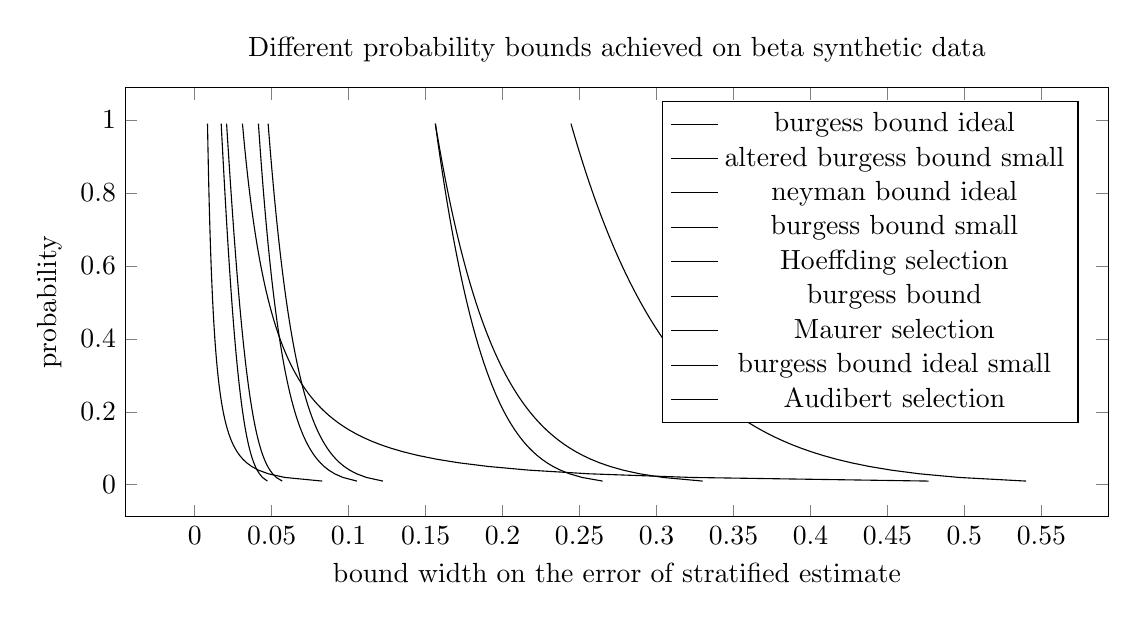
\begin{tikzpicture}
		\begin{axis}[
			title={Different probability bounds achieved on beta synthetic data},
			xlabel={bound width on the error of stratified estimate},
			ylabel={probability},
			xticklabel style={/pgf/number format/fixed},
			legend pos=north east,
			width=400,
			height=200,
		]
		\addplot[black] coordinates {
(0.0472384761849,0.01)(0.0440402461361,0.02)(0.0420568064726,0.03)(0.0405907985532,0.04)(0.0394161432024,0.05)(0.0384297361184,0.06)(0.0375755441765,0.07)(0.0368195949821,0.08)(0.0361396777665,0.09)(0.0355204447102,0.1)(0.0349508303227,0.11)(0.0344225836564,0.12)(0.0339293819689,0.13)(0.0334662691022,0.14)(0.0330292852382,0.15)(0.03261521458,0.16)(0.0322214084735,0.17)(0.0318456583622,0.18)(0.0314861025803,0.19)(0.031141156688,0.2)(0.0308094605366,0.21)(0.0304898374496,0.22)(0.0301812623276,0.23)(0.029882836429,0.24)(0.0295937672092,0.25)(0.0293133520473,0.26)(0.0290409649885,0.27)(0.0287760458555,0.28)(0.0285180912355,0.29)(0.0282666469679,0.3)(0.0280213018401,0.31)(0.0277816822665,0.32)(0.02754744777,0.33)(0.0273182871256,0.34)(0.0270939150519,0.35)(0.0268740693602,0.36)(0.0266585084858,0.37)(0.0264470093423,0.38)(0.0262393654494,0.39)(0.0260353852924,0.4)(0.0258348908803,0.41)(0.0256377164743,0.42)(0.0254437074625,0.43)(0.0252527193616,0.44)(0.0250646169279,0.45)(0.0248792733645,0.46)(0.0246965696114,0.47)(0.024516393709,0.48)(0.024338640226,0.49)(0.0241632097431,0.5)(0.0239900083871,0.51)(0.0238189474096,0.52)(0.023649942804,0.53)(0.0234829149579,0.54)(0.0233177883369,0.55)(0.0231544911957,0.56)(0.0229929553144,0.57)(0.022833115757,0.58)(0.02267491065,0.59)(0.0225182809793,0.6)(0.022363170403,0.61)(0.0222095250798,0.62)(0.0220572935093,0.63)(0.0219064263862,0.64)(0.021756876464,0.65)(0.0216085984297,0.66)(0.0214615487871,0.67)(0.0213156857486,0.68)(0.0211709691343,0.69)(0.0210273602789,0.7)(0.0208848219438,0.71)(0.0207433182359,0.72)(0.0206028145314,0.73)(0.0204632774047,0.74)(0.0203246745614,0.75)(0.020186974776,0.76)(0.0200501478332,0.77)(0.0199141644726,0.78)(0.019778996337,0.79)(0.0196446159234,0.8)(0.0195109965368,0.81)(0.0193781122468,0.82)(0.0192459378468,0.83)(0.0191144488142,0.84)(0.0189836212746,0.85)(0.018853431966,0.86)(0.0187238582058,0.87)(0.0185948778596,0.88)(0.0184664693104,0.89)(0.0183386114306,0.9)(0.0182112835539,0.91)(0.0180844654497,0.92)(0.0179581372978,0.93)(0.0178322796643,0.94)(0.0177068734782,0.95)(0.0175819000097,0.96)(0.0174573408484,0.97)(0.0173331778825,0.98)(0.0172093932792,0.99)
        };
\addlegendentry{burgess bound ideal};
		\addplot[black] coordinates {
(0.476754272664,0.01)(0.322493615139,0.02)(0.256045244224,0.03)(0.217150655845,0.04)(0.190971424239,0.05)(0.171861602357,0.06)(0.157149026364,0.07)(0.14538632911,0.08)(0.135713498578,0.09)(0.127583676042,0.1)(0.120630597012,0.11)(0.114598660397,0.12)(0.109303439954,0.13)(0.104608133993,0.14)(0.100408875445,0.15)(0.0966252177351,0.16)(0.0931937726802,0.17)(0.0900638374477,0.18)(0.0871943158149,0.19)(0.0845515045482,0.2)(0.0821074718485,0.21)(0.0798388495836,0.22)(0.077725920182,0.23)(0.0757519169303,0.24)(0.0739024811988,0.25)(0.0721652366769,0.26)(0.0705294519679,0.27)(0.0689857706847,0.28)(0.0675259936662,0.29)(0.0661429018395,0.3)(0.0648301110655,0.31)(0.0635819523716,0.32)(0.0623933724904,0.33)(0.0612598507644,0.34)(0.0601773293289,0.35)(0.0591421541419,0.36)(0.058151024925,0.37)(0.0572009524696,0.38)(0.0562892220626,0.39)(0.0554133620228,0.4)(0.054571116526,0.41)(0.0537604220461,0.42)(0.0529793868568,0.43)(0.0522262731371,0.44)(0.0514994812973,0.45)(0.0507975362091,0.46)(0.0501190750715,0.47)(0.0494628366893,0.48)(0.0488276519729,0.49)(0.0482124354994,0.5)(0.0476161779977,0.51)(0.0470379396405,0.52)(0.0464768440425,0.53)(0.04593207288,0.54)(0.0454028610559,0.55)(0.0448884923467,0.56)(0.0443882954761,0.57)(0.0439016405662,0.58)(0.0434279359246,0.59)(0.0429666251302,0.6)(0.0425171843857,0.61)(0.0420791201084,0.62)(0.0416519667344,0.63)(0.0412352847141,0.64)(0.0408286586802,0.65)(0.0404316957702,0.66)(0.0400440240884,0.67)(0.0396652912949,0.68)(0.0392951633078,0.69)(0.0389333231093,0.7)(0.0385794696459,0.71)(0.0382333168127,0.72)(0.0378945925169,0.73)(0.0375630378104,0.74)(0.037238406088,0.75)(0.0369204623439,0.76)(0.0366089824821,0.77)(0.0363037526762,0.78)(0.0360045687749,0.79)(0.0357112357474,0.8)(0.0354235671693,0.81)(0.0351413847412,0.82)(0.0348645178412,0.83)(0.0345928031064,0.84)(0.0343260840421,0.85)(0.0340642106561,0.86)(0.0338070391169,0.87)(0.033554431433,0.88)(0.0333062551527,0.89)(0.0330623830824,0.9)(0.0328226930219,0.91)(0.0325870675163,0.92)(0.0323553936224,0.93)(0.0321275626886,0.94)(0.0319034701487,0.95)(0.0316830153266,0.96)(0.0314661012532,0.97)(0.0312526344928,0.98)(0.0310425249799,0.99)
        };
\addlegendentry{altered burgess bound small}
		\addplot[black] coordinates {
(0.0828647212944,0.01)(0.0585942063484,0.02)(0.0478419691457,0.03)(0.0414323606472,0.04)(0.0370582299502,0.05)(0.0338293808082,0.06)(0.0313199207151,0.07)(0.0292971031742,0.08)(0.0276215737648,0.09)(0.0262041256965,0.1)(0.0249846535355,0.11)(0.0239209845728,0.12)(0.0229825385811,0.13)(0.0221465283239,0.14)(0.0213955790374,0.15)(0.0207161803236,0.16)(0.0200976469726,0.17)(0.0195314021161,0.18)(0.0190104708477,0.19)(0.0185291149751,0.2)(0.0180825646559,0.21)(0.0176668179406,0.22)(0.0172784888067,0.23)(0.0169146904041,0.24)(0.0165729442589,0.25)(0.0162511088796,0.26)(0.0159473230486,0.27)(0.0156599603576,0.28)(0.0153875924437,0.29)(0.0151289590248,0.3)(0.0148829432955,0.31)(0.0146485515871,0.32)(0.0144248964444,0.33)(0.0142111824602,0.34)(0.0140066943538,0.35)(0.0138107868824,0.36)(0.0136228762641,0.37)(0.01344243285,0.38)(0.0132689748365,0.39)(0.0131020628483,0.4)(0.0129412952524,0.41)(0.0127863040894,0.42)(0.0126367515284,0.43)(0.0124923267678,0.44)(0.0123527433167,0.45)(0.0122177366039,0.46)(0.0120870618671,0.47)(0.0119604922864,0.48)(0.0118378173278,0.49)(0.0117188412697,0.5)(0.0116033818897,0.51)(0.0114912692905,0.52)(0.0113823448485,0.53)(0.0112764602694,0.54)(0.01117347674,0.55)(0.0110732641619,0.56)(0.0109757004614,0.57)(0.0108806709631,0.58)(0.0107880678241,0.59)(0.0106977895187,0.6)(0.010609740371,0.61)(0.0105238301282,0.62)(0.0104399735717,0.63)(0.0103580901618,0.64)(0.0102781037126,0.65)(0.0101999420937,0.66)(0.0101235369573,0.67)(0.0100488234863,0.68)(0.00997574016375,0.69)(0.00990422855956,0.7)(0.00983423313436,0.71)(0.00976570105807,0.72)(0.00969858204239,0.73)(0.00963282818564,0.74)(0.00956839382913,0.75)(0.00950523542387,0.76)(0.00944331140688,0.77)(0.00938258208625,0.78)(0.0093230095342,0.79)(0.00926455748755,0.8)(0.00920719125494,0.81)(0.00915087763031,0.82)(0.00909558481214,0.83)(0.00904128232793,0.84)(0.00898794096371,0.85)(0.00893553269791,0.86)(0.00888403063956,0.87)(0.00883340897029,0.88)(0.00878364288994,0.89)(0.00873470856552,0.9)(0.00868658308321,0.91)(0.00863924440336,0.92)(0.00859267131796,0.93)(0.00854684341084,0.94)(0.00850174101997,0.95)(0.00845734520205,0.96)(0.00841363769912,0.97)(0.00837060090692,0.98)(0.00832821784518,0.99)
        };
\addlegendentry{neyman bound ideal}
		\addplot[black] coordinates {
(0.122278188928,0.01)(0.111525697345,0.02)(0.105195023775,0.03)(0.100681403956,0.04)(0.0971661106301,0.05)(0.0942836676561,0.06)(0.0918387712868,0.07)(0.0897146634202,0.08)(0.087835929991,0.09)(0.0861510152997,0.1)(0.084623105181,0.11)(0.0832249889386,0.12)(0.0819359822506,0.13)(0.0807399920761,0.14)(0.0796242498168,0.15)(0.0785784535437,0.16)(0.0775941703154,0.17)(0.0766644093125,0.18)(0.0757833103442,0.19)(0.0749459122073,0.2)(0.0741479775208,0.21)(0.073385858272,0.22)(0.0726563912191,0.23)(0.0719568155293,0.24)(0.0712847072076,0.25)(0.0706379263694,0.26)(0.0700145744489,0.27)(0.0694129591772,0.28)(0.0688315656967,0.29)(0.0682690325635,0.3)(0.0677241316782,0.31)(0.0671957513965,0.32)(0.0666828822347,0.33)(0.0661846047036,0.34)(0.0657000789038,0.35)(0.0652285355831,0.36)(0.064769268416,0.37)(0.0643216273121,0.38)(0.0638850125899,0.39)(0.0634588698883,0.4)(0.0630426857038,0.41)(0.0626359834648,0.42)(0.0622383200666,0.43)(0.061849282804,0.44)(0.0614684866471,0.45)(0.0610955718168,0.46)(0.0607302016197,0.47)(0.0603720605101,0.48)(0.0600208523526,0.49)(0.059676298858,0.5)(0.0593381381754,0.51)(0.0590061236192,0.52)(0.0586800225182,0.53)(0.0583596151711,0.54)(0.0580446938981,0.55)(0.0577350621779,0.56)(0.0574305338599,0.57)(0.057130932446,0.58)(0.0568360904324,0.59)(0.0565458487079,0.6)(0.0562600560004,0.61)(0.0559785683692,0.62)(0.0557012487375,0.63)(0.0554279664618,0.64)(0.0551585969342,0.65)(0.0548930212151,0.66)(0.0546311256941,0.67)(0.0543728017746,0.68)(0.0541179455831,0.69)(0.0538664576972,0.7)(0.0536182428953,0.71)(0.0533732099214,0.72)(0.0531312712679,0.73)(0.052892342972,0.74)(0.0526563444262,0.75)(0.0524231982012,0.76)(0.0521928298805,0.77)(0.0519651679053,0.78)(0.0517401434295,0.79)(0.0515176901838,0.8)(0.0512977443481,0.81)(0.0510802444318,0.82)(0.0508651311611,0.83)(0.0506523473735,0.84)(0.0504418379179,0.85)(0.0502335495613,0.86)(0.0500274309,0.87)(0.0498234322763,0.88)(0.0496215057003,0.89)(0.0494216047752,0.9)(0.0492236846272,0.91)(0.0490277018396,0.92)(0.0488336143891,0.93)(0.0486413815876,0.94)(0.0484509640246,0.95)(0.0482623235151,0.96)(0.0480754230479,0.97)(0.0478902267383,0.98)(0.0477066997823,0.99)
        };
\addlegendentry{burgess bound small}
		\addplot[black] coordinates {
(0.264970774769,0.01)(0.251627381778,0.02)(0.24348163752,0.03)(0.237531865556,0.04)(0.232811542638,0.05)(0.228882030947,0.06)(0.225505886171,0.07)(0.222539629828,0.08)(0.219889732857,0.09)(0.217491736012,0.1)(0.215299276634,0.11)(0.213277860713,0.12)(0.211401109412,0.13)(0.209648384982,0.14)(0.208003228272,0.15)(0.206452295573,0.16)(0.204984614426,0.17)(0.203591049838,0.18)(0.202263913189,0.19)(0.200996670286,0.2)(0.199783719796,0.21)(0.198620222584,0.22)(0.197501968514,0.23)(0.196425271231,0.24)(0.195386884148,0.25)(0.194383932685,0.26)(0.193413859127,0.27)(0.192474377376,0.28)(0.191563435526,0.29)(0.190679184703,0.3)(0.189819952935,0.31)(0.188984223112,0.32)(0.188170614294,0.33)(0.187377865764,0.34)(0.186604823356,0.35)(0.185850427687,0.36)(0.185113703976,0.37)(0.184393753193,0.38)(0.183689744353,0.39)(0.183000907756,0.4)(0.182326529062,0.41)(0.181665944062,0.42)(0.181018534054,0.43)(0.180383721749,0.44)(0.179760967618,0.45)(0.179149766649,0.46)(0.178549645434,0.47)(0.177960159568,0.48)(0.177380891303,0.49)(0.176811447441,0.5)(0.176251457431,0.51)(0.175700571649,0.52)(0.175158459834,0.53)(0.174624809674,0.54)(0.174099325517,0.55)(0.173581727195,0.56)(0.173071748952,0.57)(0.172569138465,0.58)(0.172073655942,0.59)(0.171585073301,0.6)(0.171103173412,0.61)(0.170627749401,0.62)(0.170158604007,0.63)(0.169695548989,0.64)(0.169238404584,0.65)(0.168786998993,0.66)(0.168341167919,0.67)(0.167900754133,0.68)(0.167465607063,0.69)(0.167035582428,0.7)(0.166610541885,0.71)(0.166190352704,0.72)(0.165774887469,0.73)(0.165364023789,0.74)(0.164957644041,0.75)(0.164555635119,0.76)(0.164157888205,0.77)(0.163764298554,0.78)(0.163374765287,0.79)(0.162989191204,0.8)(0.162607482607,0.81)(0.162229549129,0.82)(0.161855303576,0.83)(0.161484661783,0.84)(0.161117542468,0.85)(0.160753867105,0.86)(0.160393559797,0.87)(0.160036547161,0.88)(0.159682758212,0.89)(0.159332124266,0.9)(0.158984578833,0.91)(0.158640057529,0.92)(0.158298497984,0.93)(0.157959839759,0.94)(0.157624024266,0.95)(0.157290994694,0.96)(0.156960695932,0.97)(0.156633074507,0.98)(0.156308078517,0.99)
        };
\addlegendentry{Hoeffding selection}
		\addplot[black] coordinates {
(0.105403711005,0.01)(0.0963000445963,0.02)(0.0909260373623,0.03)(0.0870890161098,0.04)(0.0840964200915,0.05)(0.0816392406465,0.06)(0.0795529424313,0.07)(0.0777381436033,0.08)(0.0761316158742,0.09)(0.0746897186479,0.1)(0.0733810230785,0.11)(0.0721826694502,0.12)(0.0710771480032,0.13)(0.0700508994277,0.14)(0.0690930425389,0.15)(0.0681947326428,0.16)(0.0673487281484,0.17)(0.0665491253061,0.18)(0.0657907977869,0.19)(0.0650694265194,0.2)(0.0643818150162,0.21)(0.0637249100389,0.22)(0.0630960444419,0.23)(0.0624927569742,0.24)(0.0619129695785,0.25)(0.0613548683952,0.26)(0.060816688868,0.27)(0.0602970843389,0.28)(0.0597945966142,0.29)(0.0593082826185,0.3)(0.0588370667637,0.31)(0.0583799180685,0.32)(0.0579360585258,0.33)(0.0575046264412,0.34)(0.0570849912996,0.35)(0.0566765561473,0.36)(0.0562784774127,0.37)(0.0558902258099,0.38)(0.0555114893596,0.39)(0.0551415032187,0.4)(0.0547800104885,0.41)(0.054426727548,0.42)(0.0540812711171,0.43)(0.0537431967521,0.44)(0.0534122014721,0.45)(0.0530879851722,0.46)(0.052770302575,0.47)(0.0524588133596,0.48)(0.0521532303791,0.49)(0.051853282316,0.5)(0.0515588597215,0.51)(0.0512697491136,0.52)(0.0509857243728,0.53)(0.0507066105769,0.54)(0.0504321893626,0.55)(0.0501623075208,0.56)(0.0498968314349,0.57)(0.049635619919,0.58)(0.0493785007502,0.59)(0.0491252977118,0.6)(0.0488759423968,0.61)(0.048630333694,0.62)(0.0483883397025,0.63)(0.0481498494444,0.64)(0.0479147189805,0.65)(0.0476828756275,0.66)(0.0474542032888,0.67)(0.0472285829771,0.68)(0.0470059481113,0.69)(0.0467862489652,0.7)(0.0465693982656,0.71)(0.0463552892743,0.72)(0.0461438750414,0.73)(0.0459350733872,0.74)(0.0457288154679,0.75)(0.0455250089989,0.76)(0.0453235981153,0.77)(0.0451244963545,0.78)(0.0449276783879,0.79)(0.0447330172477,0.8)(0.0445404922798,0.81)(0.0443500798008,0.82)(0.0441617391138,0.83)(0.043975421965,0.84)(0.0437910733405,0.85)(0.0436086410699,0.86)(0.0434280858889,0.87)(0.0432493186496,0.88)(0.0430723325921,0.89)(0.0428970955865,0.9)(0.0427235927615,0.91)(0.0425517710195,0.92)(0.0423815985561,0.93)(0.0422130474639,0.94)(0.0420460417544,0.95)(0.0418805786913,0.96)(0.0417166280825,0.97)(0.0415541708025,0.98)(0.0413931663492,0.99)
        };
\addlegendentry{burgess bound}
		\addplot[black] coordinates {
(0.540127229671,0.01)(0.49644611748,0.02)(0.470785478605,0.03)(0.452525133511,0.04)(0.438328295384,0.05)(0.42670599844,0.06)(0.416862848225,0.07)(0.408323494545,0.08)(0.400781006338,0.09)(0.394025618503,0.1)(0.387907588562,0.11)(0.382316267369,0.12)(0.377167567245,0.13)(0.372396082469,0.14)(0.367949931729,0.15)(0.36378726656,0.16)(0.359873838874,0.17)(0.356181263975,0.18)(0.352685753237,0.19)(0.349367171812,0.2)(0.346208326183,0.21)(0.343194417382,0.22)(0.340312615688,0.23)(0.337551725782,0.24)(0.334901920208,0.25)(0.332354525068,0.26)(0.329901846119,0.27)(0.327537026477,0.28)(0.325253929258,0.29)(0.323047040092,0.3)(0.320911385613,0.31)(0.318842464865,0.32)(0.316836191253,0.33)(0.314888843156,0.34)(0.312997021674,0.35)(0.311157614339,0.36)(0.309367763773,0.37)(0.307624840534,0.38)(0.305926419473,0.39)(0.304270259091,0.4)(0.302654283431,0.41)(0.301076566152,0.42)(0.29953531648,0.43)(0.298028866765,0.44)(0.296555661434,0.45)(0.295114247158,0.46)(0.293703264081,0.47)(0.292321437955,0.48)(0.290967573106,0.49)(0.289640546086,0.5)(0.288339299974,0.51)(0.287062839216,0.52)(0.285810224959,0.53)(0.284580570823,0.54)(0.283373039056,0.55)(0.28218683704,0.56)(0.2810212141,0.57)(0.279875458594,0.58)(0.278748895252,0.59)(0.277640882732,0.6)(0.276550811386,0.61)(0.275478101203,0.62)(0.274422199914,0.63)(0.273382581252,0.64)(0.272358743339,0.65)(0.271350207204,0.66)(0.270356515409,0.67)(0.269377230772,0.68)(0.268411935189,0.69)(0.26746022854,0.7)(0.266521727669,0.71)(0.265596065438,0.72)(0.264682889847,0.73)(0.263781863211,0.74)(0.26289266139,0.75)(0.26201497308,0.76)(0.261148499138,0.77)(0.260292951957,0.78)(0.259448054884,0.79)(0.258613541661,0.8)(0.257789155921,0.81)(0.256974650695,0.82)(0.256169787962,0.83)(0.255374338219,0.84)(0.254588080081,0.85)(0.253810799902,0.86)(0.253042291415,0.87)(0.252282355399,0.88)(0.251530799362,0.89)(0.250787437236,0.9)(0.250052089099,0.91)(0.249324580905,0.92)(0.248604744231,0.93)(0.247892416035,0.94)(0.247187438432,0.95)(0.246489658477,0.96)(0.245798927962,0.97)(0.245115103218,0.98)(0.244438044938,0.99)
        };
\addlegendentry{Maurer selection}
		\addplot[black] coordinates {
(0.0568733355696,0.01)(0.0530227877644,0.02)(0.0506348015574,0.03)(0.0488697835662,0.04)(0.0474555430288,0.05)(0.0462679462723,0.06)(0.0452395315377,0.07)(0.0443293973488,0.08)(0.0435108027817,0.09)(0.0427652696432,0.1)(0.042079475502,0.11)(0.0414434865299,0.12)(0.0408496903844,0.13)(0.0402921200392,0.14)(0.0397660080233,0.15)(0.039267482639,0.16)(0.0387933550072,0.17)(0.0383409661094,0.18)(0.0379080745707,0.19)(0.0374927727856,0.2)(0.0370934231866,0.21)(0.0367086090996,0.22)(0.036337096344,0.23)(0.0359778028686,0.24)(0.0356297744802,0.25)(0.0352921652495,0.26)(0.0349642215509,0.27)(0.0346452689519,0.28)(0.0343347013627,0.29)(0.0340319719911,0.3)(0.0337365857529,0.31)(0.0334480928649,0.32)(0.0331660834057,0.33)(0.0328901826722,0.34)(0.0326200471965,0.35)(0.0323553613131,0.36)(0.0320958341874,0.37)(0.0318411972318,0.38)(0.0315912018519,0.39)(0.0313456174712,0.4)(0.0311042297953,0.41)(0.030866839281,0.42)(0.0306332597814,0.43)(0.030403317344,0.44)(0.0301768491406,0.45)(0.0299537025125,0.46)(0.0297337341159,0.47)(0.029516809156,0.48)(0.0293028006971,0.49)(0.0290915890423,0.5)(0.0288830611719,0.51)(0.0286771102361,0.52)(0.0284736350941,0.53)(0.0282725398957,0.54)(0.0280737337003,0.55)(0.0278771301293,0.56)(0.0276826470484,0.57)(0.0274902062773,0.58)(0.0272997333225,0.59)(0.0271111571332,0.6)(0.0269244098762,0.61)(0.0267394267283,0.62)(0.0265561456851,0.63)(0.0263745073849,0.64)(0.0261944549447,0.65)(0.0260159338094,0.66)(0.0258388916111,0.67)(0.025663278039,0.68)(0.0254890447184,0.69)(0.0253161450975,0.7)(0.0251445343425,0.71)(0.0249741692394,0.72)(0.0248050081027,0.73)(0.0246370106888,0.74)(0.0244701381168,0.75)(0.0243043527923,0.76)(0.0241396183372,0.77)(0.0239758995232,0.78)(0.0238131622092,0.79)(0.0236513732825,0.8)(0.0234905006036,0.81)(0.0233305129532,0.82)(0.0231713799832,0.83)(0.0230130721699,0.84)(0.0228555607689,0.85)(0.0226988177739,0.86)(0.022542815876,0.87)(0.0223875284259,0.88)(0.0222329293978,0.89)(0.0220789933546,0.9)(0.0219256954153,0.91)(0.0217730112227,0.92)(0.0216209169141,0.93)(0.0214693890918,0.94)(0.0213184047951,0.95)(0.021167941474,0.96)(0.021017976963,0.97)(0.0208684894564,0.98)(0.0207194574838,0.99)
        };
\addlegendentry{burgess bound ideal small}
		\addplot[black] coordinates {
(0.329972885371,0.01)(0.304193433079,0.02)(0.289063362072,0.03)(0.278303781683,0.04)(0.269942964053,0.05)(0.263101402999,0.06)(0.257309414943,0.07)(0.252286375452,0.08)(0.247851127268,0.09)(0.243879887197,0.1)(0.240284307557,0.11)(0.236999116427,0.12)(0.233974718072,0.13)(0.231172541057,0.14)(0.228561993729,0.15)(0.226118403373,0.16)(0.223821580662,0.17)(0.221654794643,0.18)(0.219604024966,0.19)(0.217657405941,0.2)(0.215804806238,0.21)(0.214037506351,0.22)(0.21234794774,0.23)(0.210729535345,0.24)(0.209176480392,0.25)(0.207683674023,0.26)(0.206246584751,0.27)(0.204861174562,0.28)(0.203523829718,0.29)(0.202231303294,0.3)(0.20098066712,0.31)(0.199769271351,0.32)(0.198594710254,0.33)(0.197454793094,0.34)(0.196347519237,0.35)(0.19527105676,0.36)(0.194223723987,0.37)(0.193203973481,0.38)(0.192210378119,0.39)(0.191241618924,0.4)(0.190296474401,0.41)(0.189373811154,0.42)(0.188472575604,0.43)(0.187591786667,0.44)(0.186730529239,0.45)(0.185887948411,0.46)(0.185063244298,0.47)(0.184255667408,0.48)(0.1834645145,0.49)(0.182689124846,0.5)(0.181928876873,0.51)(0.181183185125,0.52)(0.180451497517,0.53)(0.179733292844,0.54)(0.179028078516,0.55)(0.178335388504,0.56)(0.177654781457,0.57)(0.176985838993,0.58)(0.176328164129,0.59)(0.175681379845,0.6)(0.175045127767,0.61)(0.174419066956,0.62)(0.173802872796,0.63)(0.173196235963,0.64)(0.172598861483,0.65)(0.172010467857,0.66)(0.171430786247,0.67)(0.170859559734,0.68)(0.170296542618,0.69)(0.169741499778,0.7)(0.169194206066,0.71)(0.168654445758,0.72)(0.168122012031,0.73)(0.16759670648,0.74)(0.167078338665,0.75)(0.166566725694,0.76)(0.166061691826,0.77)(0.165563068104,0.78)(0.165070692008,0.79)(0.164584407134,0.8)(0.164104062891,0.81)(0.163629514214,0.82)(0.163160621298,0.83)(0.162697249346,0.84)(0.162239268333,0.85)(0.161786552782,0.86)(0.161338981558,0.87)(0.160896437662,0.88)(0.160458808054,0.89)(0.16002598347,0.9)(0.159597858255,0.91)(0.159174330212,0.92)(0.158755300445,0.93)(0.158340673223,0.94)(0.157930355844,0.95)(0.157524258512,0.96)(0.157122294211,0.97)(0.156724378596,0.98)(0.156330429881,0.99)
        };
\addlegendentry{Audibert selection}
\end{axis}
\end{tikzpicture}
	\caption{Different probability bound widths for the beta-distributed data (per section \ref{sec:beta_distributed_data}) at $n=50N$}
	\label{fig:bounds_widths}
\end{figure}


%Next, note that the results of Figure~\ref{Table1} show that there is a mid-range of sample sizes where choosing a different method can even have a greater impact on sampling efficiency and rate of average error reduction than the difference between sampling with or without replacement.
%This is an important insight, as sampling real-world data (e.g. surveys, polling, destructive testing, etc) can be an expensive and slow process.
%Accordingly an appropriate method of choosing numbers of samples can lead to a material difference in cost for the same accuracy.
%There is also a slight decrease in the performance of SEBM* in comparison with \textsc{Ney} in the case of high number of samples and sampling without replacement, as illustrated in Figure~\ref{Table1}. 
%This indicates that the use of sub-optimal equation~\ref{approx1} in the derivation of Lemma~\ref{martingale0} might have some negative effect, by distorting the shape of the functions that the sampling processes then minimizes.

%If the data features very rare events, then SEBM and SEBM* seem to perform in a manner less than ideal.
%These condition are illustrated in Figure~\ref{biggraph3}, where the more rare the Bernoulli variable successes, the worse our methods perform in comparison with Neyman sampling (\textsc{Ney}).
%This shortcoming can be partly explained by noting that SEBM unnecessarily wastes samples on the Bernoulli stratum of rare events in the process of learning that the variance is almost zero, whereas \textsc{Ney} can avoid this because it has prior knowledge of the variances to begin with. 
%As such, this factor explains the difference between the performance of SEBM and SEBM* in the context of Figure~\ref{Table1} and also in Figure~\ref{biggraph3}.
%What is surprising is how small the difference in performance between SEBM and SEBM* is. 
%This indicates that as additional samples are taken, the original uncertainty about the strata variances have less and less effect upon the total numbers of samples that are eventually drawn from each of the strata.

%However, the performance difference between SEBM* and \textsc{Ney} in Figure~\ref{biggraph3} is not explained by this argument, as they use the same information.
%Instead, the reason for this difference in performance is found by considering the simplifying approximation of Equation \eqref{eq:part2} in the derivation of Lemma~\ref{expectation1}. 
%Specifically, \eqref{eq:part2} introduces a particular distortion into the shape of Equation~\eqref{big_equation} which our sampling seeks to minimize.
%Figure~\ref{fig:graph2} illustrates how the approximation \eqref{eq:part2} loosens the bound with respect to the variance. 
%Observe that when the variances are very small that Equation~\eqref{eq:part3} overly loosens the bounds, causing oversampling of strata with very small variances. 
%It appears that this factor is at play in the under-performance shown in Figure~\ref{biggraph3} and also the slight under-performance of our method in the Voting Game in Table~\ref{tab2}. 
%We note that there may be other corner-cases where our method also under-performs.

\subsection{Discussion of Shapley Value results}\label{subsection:discussion_shapley}

In considering the comparison of approaches to approximating the Shapley value, our sampling method (SEBM, with error $e^{SEBM}$) shows improved performance on almost all accounts, as shown in Table~\ref{Table2}.
This was particularly the case in the context of large sample budgets, as our method sampled without replacement, while the other methods sampled with replacement.
Additionally we also note that our method's performance could potentially be further improved by selecting more refined $D_i$ values in the context of our example games.

We additionally attribute our methods success in estimating the Shapley Value primarily to the design decisions used in the creation of those other methods.
Particularly we note that Castro's Neyman sampling method (with error $e^{Ca}$) deploys about half the samples learning about the variance and the other half using a Neyman style allocation.
The choice of allocating half the samples was identified as a default by Castro with the acknowledgement that the proportion should be treated as a context dependant parameter.
However, to make a fair comparison with other methods we did not tune any context dependant parameter for any of the methods.

In the process of generating these results one of the major effects that was witnessed in our sampling method (SEBM) was the computational overhead of iteratively minimising (one sample at a time) our inequality (equation \ref{big_equation}) in the context of our simple example games.
Although we acknowledged and expected a computational overhead, we designed our method with the intention of using it to approximate the GNK value (per section \ref{sec:sampling_techniques}), where each additional sample requires running an optimisation problem, and in this context a computational overhead about which sample to choose was deemed less relevant.


%\input{figure-22.tex} 

One primary limitation of our method(s) is that it rests on assumption of known data widths $D_i$ (and in the case of sampling-without-replacement, also on strata sizes $N_i$), which may not be exactly known in practice.
One way to overcome this may be to use our method with a reliable overestimate these parameters (by expert opinion or otherwise). This approximation or estimation may itself open consideration of other probability bounds and/or sampling methods, however we have not investigated this line of inquiry. 
In practice, it might also be advisable to run our method with an underestimate of the data widths, as the sampling process is fundamentally sensitive the the shape of the inequality and not necessarily its magnitude or accuracy as a bound.

% Our concentration inequality, Equation~\eqref{big_equation}, is derived by a combination of Chernoff bounds fused together with probability unions, so it is expected to give conservative confidence intervals on the error of the estimate in stratified random sampling, which may be useful outside of the context of sampling decisions.







\subsection{Future Work: applications of a Multidimensional Extension}\label{sec:multi}

It was noticed that our SEBB can be extended to multidimensional data by a simple modification.
Specifically, instead of considering data that is single-valued, we consider data points that are vectors. 

Formally, for $n$ strata of finite data points which are all vectors of size $M$, let $n_i$ be the number of data points in the $i$th stratum.
Let the data in the $i$th stratum have a mean vector values $\mu_i$ (with $\mu_{i,j}$ for the $j$th component of the vector), which are value bounded within a finite width $D_{i,j}$, and have vector value variances $\sigma_{i,j}^2$.  
Given this, let $X_{i,1},X_{i,2},\dots,X_{i,n_i}$ (where $X_{i,k,j}$ is the $j$th component, of the $k$th vector from stratum $i$) be vector random variables corresponding to those data values randomly and sequentially drawn (with or without) replacement. 
Denote the average of the first $m_i$ of these random variables from the $i$th stratum by $\chi_{i,m_i}= \frac{1}{m_i}\sum_{k=1}^{m_i}X_{i,k}$ (with $\chi_{i,m_i,j}$ being the $j$th component of that vector average).
Let $\doublehat{\sigma}_{i,j}^2=\frac{i}{m_i-1}\sum_{k=1}^{m_i}(X_{i,k,j}-\chi_{i,m_i,j})^2$ be the unbiased sample variance of the first $m_i$ of these random variables in the $j$th component. 
As before, we assume weights $\tau_i$ for each stratum. \\
In this context we have the following theorem:

\begin{theorem}[Vector SEBM bound]
In the context above, then with $\Omega_{m_i}^{n_i},\Psi_{m_i}^{n_i}$ per Lemma~\ref{martingale1}:
%\begin{equation}\label{big_equation2}\p\left(\begin{matrix*}[l]\sum_{j=1}^M\left(\sum_{i=1}^n\tau_i(\chi_{i,m_i,j}-\mu_{i,j})\right)^2 \ge \\ \quad\quad \log(6/p)\sum_{j=1}^M\begin{pmatrix*}[l]\sum_{i=1}^n\frac{4}{17}\Omega_{m_i}^{n_i}D_{i,j}^2\tau_i^2 \\ +\begin{pmatrix*}[l]\sqrt{\log(3/p)\left(\max_i\tau_i^2{\Psi_{m_i}^{n_i}}^2D_{i,j}^2\right)} \\ +\sqrt{\begin{matrix*}[l]2\sum_{i=1}^n\tau_i^2\Psi_{m_i}^{n_i}(m_i-1)\doublehat{\sigma}_{i,j}^2/m_i \\ + \log(6n/p)\sum_i\tau_i^2D_{i,j}^2\Omega_{m_i}^{n_i}\Psi_{m_i}^{n_i} \\ +\log(3/p)\left(\max_i\tau_i^2{\Psi_{m_i}^{n_i}}^2D_{i,j}^2\right)\end{matrix*}} \end{pmatrix*}^2\end{pmatrix*}\end{matrix*} \right)\le Mp \end{equation}

\begin{equation}\label{big_equation2}\pr\left(\begin{matrix*}[l]\sum_{j=1}^M\left(\sum_{i=1}^n\tau_i(\chi_{i,m_i,j}-\mu_{i,j})\right)^2 \ge \\ \quad\quad \log(6/p)\sum_{j=1}^M\left(\alpha_{m_i,j}^{n_i} +\left(\sqrt{\beta_{m_i,j}^{n_i}} +\sqrt{\gamma_{m_i,j}^{n_i}}\right)^2\right)\end{matrix*} \right)\le Mp \end{equation}

where:

\begin{align*}
\alpha_{j}=&\sum_{i=1}^n\frac{4}{17}\Omega_{m_i}^{n_i}D_{i,j}^2\tau_i^2 \\
\beta_{j}=&\log(3/p)\left(\max_i\tau_i^2{\Psi_{m_i}^{n_i}}^2D_{i,j}^2\right) \\
\gamma_{j}=&2\sum_{i=1}^n\tau_i^2\Psi_{m_i}^{n_i}(m_i-1)\doublehat{\sigma}_{i,j}^2/m_i
+ \log(6n/p)\sum_i\tau_i^2D_{i,j}^2\Omega_{m_i}^{n_i}\Psi_{m_i}^{n_i}  \\
&\quad\quad\quad\quad\quad\quad\quad\quad\quad\quad\quad~~+\log(3/p)\left(\max_i\tau_i^2{\Psi_{m_i}^{n_i}}^2D_{i,j}^2\right)
\end{align*}

%$$
%\alpha_{m_i,j}^{n_i}
%=\sum_{i=1}^n\frac{4}{17}\Omega_{m_i}^{n_i}D_{i,j}^2\tau_i^2 
%$$
%$$
%\beta_{m_i,j}^{n_i}
%=\log(3/p)\left(\max_i\tau_i^2{\Psi_{m_i}^{n_i}}^2D_{i,j}^2\right) 
%$$
%and
%\begin{align*}
%\gamma_{m_i,j}^{n_i}
%= 2\sum_{i=1}^n\tau_i^2\Psi_{m_i}^{n_i}(m_i-1)\doublehat{\sigma}_{i,j}^2/m_i
%&+ \log(6n/p)\sum_i\tau_i^2D_{i,j}^2\Omega_{m_i}^{n_i}\Psi_{m_i}^{n_i}  \\
%&+\log(3/p)\left(\max_i\tau_i^2{\Psi_{m_i}^{n_i}}^2D_{i,j}^2\right)
%\end{align*}

\end{theorem}
\begin{proof}
Squaring \eqref{big_equation} and applying it specifically to the $j$th component of all the vectors gives:
\begin{equation*}
\pr\left(\frac{\left(\sum_{i=1}^n\tau_i(\chi_{i,m_i}-\mu_i)\right)^2}{\log(6/p)} 
\ge \alpha_{j} 
+ \left(\sqrt{\beta_{j}} 
+ \sqrt{\gamma_{j}}\right)^2  \right)
\le p 
\end{equation*}
%$$ \p\left(\frac{\left(\sum_{i=1}^n\tau_i(\chi_{i,m_i,j}-\mu_{i,j})\right)^2}{\log(6/p)}\ge \begin{matrix*}[l]\sum_{i=1}^n\frac{4}{17}\Omega_{m_i}^{n_i}D_{i,j}^2\tau_i^2 \\ +\begin{pmatrix*}[l]\sqrt{\log(3/p)\left(\max_i\tau_i^2{\Psi_{m_i}^{n_i}}^2D_{i,j}^2\right)} \\ +\sqrt{\begin{matrix*}[l]2\sum_{i=1}^n\tau_i^2\Psi_{m_i}^{n_i}(m_i-1)\doublehat{\sigma}_{i,j}^2/m_i \\ + \log(6n/p)\sum_i\tau_i^2D_{i,j}^2\Omega_{m_i}^{n_i}\Psi_{m_i}^{n_i} \\ +\log(3/p)\left(\max_i\tau_i^2{\Psi_{m_i}^{n_i}}^2D_{i,j}^2\right)\end{matrix*}} \end{pmatrix*}^2\end{matrix*} \right)\le p $$
Taking a series of union bounds (Lemma~\ref{prob_union}) over $j$ gives result.
\end{proof}

The left hand side of the inequality in \eqref{big_equation2} is the square Euclidean distance between our weighted stratified sample vector estimate $\sum_{i=1}^n\tau_i\chi_{i,m_i}$ and the true mean stratified vector $\sum_{i=1}^n\tau_i\mu_{i}$.
In this context, an example sampling process might consist of sampling to maximally minimise the right hand side of the inequality (similar to our SEBM process, described in Section~\ref{sec:SEBMalgorithm}).
This formulation can be applied to more involved computational tasks that involve sampling data with multiple features or auxiliary variables.


A potential use of this multi-dimensional stratified sampling method is in improving the performance of \textit{stochastic gradient decent} (SGD) methods for training neural networks \citep{2016arXiv160904747R}.
Neural networks are trained by iteratively refining their parameters --- the weights and biases of the network --- against a cost function of the network's performance against training data.
One common method of training neural networks is gradient decent (GD).
In each iteration of GD, the derivative of how much a change in any parameter would influence the average performance of the network across the training data is calculated as a gradient vector.
Once this vector is calculated, each network parameter takes a small step in the direction of this gradient, to incrementally increase the performance of the network, 
and through many of these steps the network becomes trained.

However in many cases, the entire corpus of training data is not used in each iteration but only a fraction of the corpus is sampled (as a `batch' or `minibatch'), and the average gradient vector of improved performance across the samples of the batch is calculated as an approximation of the true gradient vector. 
This iterative process has been called SGD, where one of the hyperparameters is the size of the batches, see \cite{DBLP:journals/corr/KeskarMNST16}.
In the context of supervised learning, each element of the training data is labelled with the desired output of the neural network for it, and these labels can serve to naturally stratify the training data; or the data can be stratified by other means too \citep{DBLP:journals/corr/ZhangKM17,DBLP:journals/corr/abs-1804-02772,2014arXiv1405.3080Z}.
In this setting, Equation~\ref{big_equation2} may be used to choose between samples of labelled training data, in order to sample batches that estimate of the performance gradient more efficiently, and hence improve the efficiency of neural network training procedure.
This idea of `smart sampling' for neural network training is not particularly new, and our method is potentially compatible with other performance-enhancing techniques in the literature on neural networks \citep{10.1007/978-3-319-24486-0_21,article123123131}.





